\section{Organizzazione fisica della base di dati}

Un requisito fondamentale di un database è l'efficienza, cioè la capacità di rispondere alle 
richieste dell'utente il più rapidamente possibile: questo obiettivo può essere raggiunto grazie
ad una particolare organizzazione fisica dei dati. In questo capitolo verrà mostrato come il database
è organizzato a livello fisico, ovvero come questo viene salvato sull'unità di memoria 
di massa (disco rigido); nel prossimo paragrafo sarà quindi necessario illustrare brevemente come il
sistema operativo gestisce la lettura e scrittura di tali dispositivi.

\subsection{La memoria secondaria}
Il computer necessita di una \emph{memoria secondaria} dove poter salvare in modo permanente
i dati presenti nella RAM. Questa memoria secondaria è tipicamente un disco rigido, la cui struttura
meccanica è illustrata nella seguente figura.
\begin{center}
 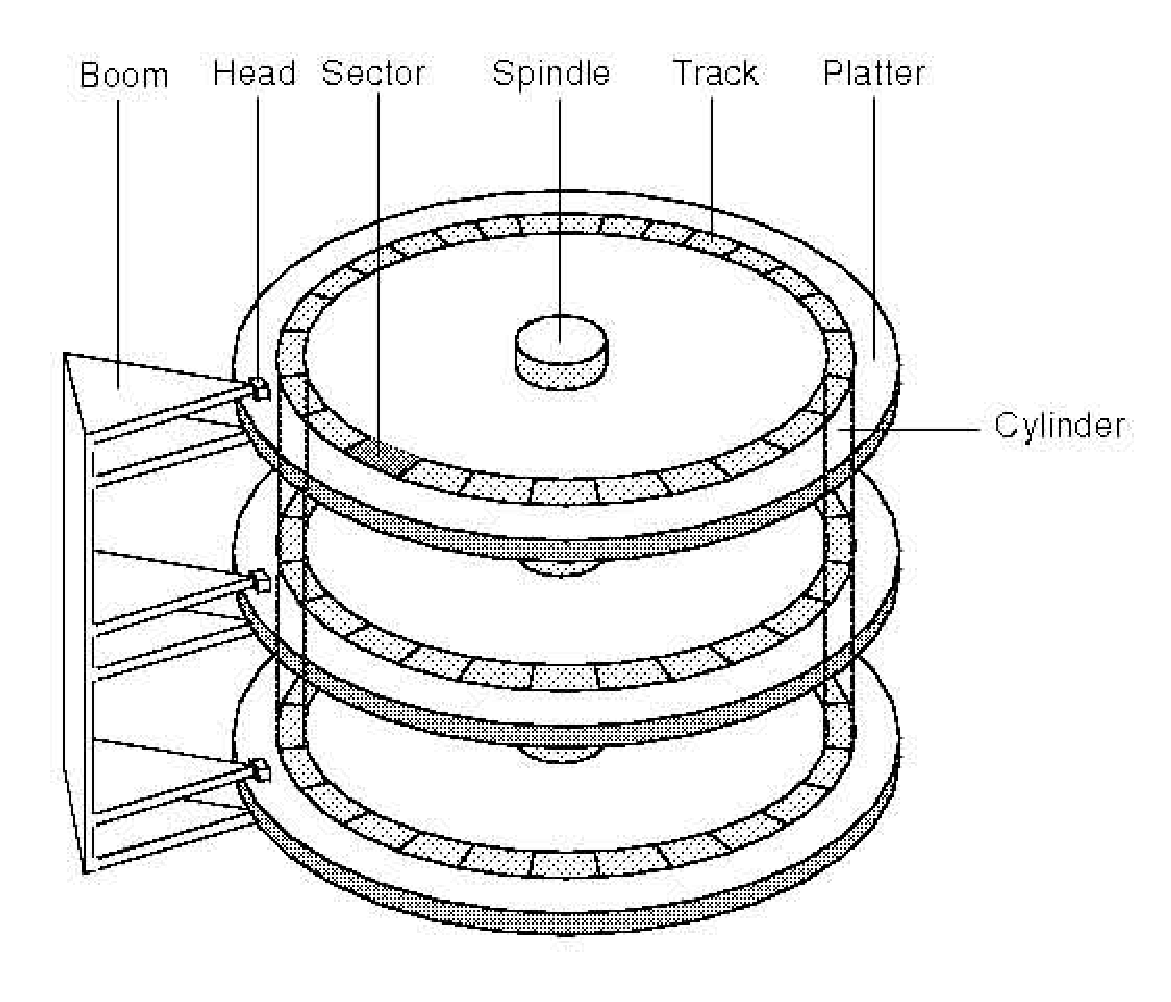
\includegraphics[width=300px]{img_5_1.eps}
\end{center}
L'unità di memoria è composta da più \textbf{piatti}, di solito tre, ognuno dei quali è suddiviso
in \textbf{tracce}: esse sono come cerchi concentrici che ripartizionano tutta la superficie del
piatto. Al momento della \emph{formattazione}, durante la quale viede data una struttura logica per 
poter memorizzare i dati, impostando la struttura del filesystem che vi verrà creato sopra, vengono
creati i \textbf{settori} (o \textbf{blocchi} o pagine) di dimensione fissa, che varia da $2^9$ a $2^{12}$
bytes.\\
Quando si parla di \emph{accesso} al disco s'intende il trasferimento di un blocco da memoria secondaria 
a memoria principale, quindi \textbf{lettura} di un blocco, o da memoria principale a memoria secondaria, 
ossia \textbf{scrittura} di un blocco. Il tempo necessario per un accesso è dato dalla somma di:
\begin{itemize}
 \item \emph{tempo di posizionamento} della testina sulla traccia in cui si trova il blocco;
 \item \emph{ritardo della rotazione}, necessaria per posizionare la testina all'inizio del blocco;
 \item \emph{tempo di trasferimento} dei dati contenuti nel blocco.
\end{itemize}
Il tempo richiesto per un accesso a memoria secondaria è dell'ordine dei millisecondi, quindi 
notevolmente superiore a quello di elaborazione dei dati in memoria principale. Per questo motivo il 
\textbf{costo} di un'operazione sulla base di dati è definito in termini di \emph{numero di accessi}.

\subsection{Memorizzare le relazioni}

\subsubsection{Record}
Ad ogni relazione corrisponde un file di record che hanno tutti lo stesso tipo (numero e 
tipo dei campi): ad ogni attributo corrisponde un \emph{campo}, che sono di tipo elementare (interi,
reali, stringhe di caratteri), ed ad ogni tupla corrisponde un record. In un record, oltre ai campi 
che corrispondono agli attributi, ci possono essere altri campi che contengono informazioni sul 
record stesso o puntatori ad altri record.\\
Un \textbf{puntatore} ad un record è essenzialmente un dato che permette di accedere rapidamente a quel
record. Pertanto un puntatore può essere l'indirizzo dell'inizio (primo byte) del record su disco.
Tale scelta però può non essere adeguata se si vuole avere una certa libertà di muovere il record; in
questo caso è preferibile assumere come puntatore una coppia $(b, k)$ in cui $b$ è l'indirizzo del blocco
che contiene il record e $k$ è il valore di uno o più campi che servono come chiave nel file a cui il
record appartiene. In tal modo è possibile spostare il record all'interno del blocco. All'inizio di un 
record alcuni byte possono essere utilizzati per:
\begin{itemize}
 \item specificare il tipo del record, necessario quando in uno stesso blocco sono memorizzati 
 record di tipo diverso;
 \item specificare la lunghezza del record, se esso ha campi a lunghezza variabile;
 \item contenere un bit di ``cancellazione'', utile nel caso che il record sia puntato. In tal caso 
 lo spazio occupato dal record cancellato non può essere riutilizzato
 \item contenere un bit di ``usato/non usato'' per specificare se in quello spazio c'è un record oppure
 è vuoto (contiene valori casuali).
\end{itemize}

Per poter accedere ad un campo di un record contenente un dato è necessario sapere qual è il primo
byte del campo nel record. Se tutti i campi del record hanno lunghezza fissa, basta ordinarli; infatti,
una volta ordinati, l'inizio di ciascun campo sarà sempre ad un numero fisso di byte dall'inizio del
record: il numero di byte del record che precedono il campo è detto \textbf{offset} del campo. Se il record
contiene campi a lunghezza variabile allora l'offset di un campo può variare da un record all'altro.
In tal caso si possono usare due strategie:
\begin{itemize}
 \item all'inizio di ogni campo c'è un contatore che specifica la lunghezza del campo in numero di
byte
\item all'inizio del record ci sono gli offset di ciascun campo a lunghezza variabile (tutti i campi 
a lunghezza fissa precedono quelli a lunghezza variabile).
\end{itemize}

Nel primo caso per individuare la posizione di un campo bisogna esaminare i campi precedenti per
vedere quanto sono lunghi; quindi la prima strategia è meno efficiente della seconda. 

\subsubsection{Blocchi}
I record sono memorizzati nei blocchi. Analogamente a quanto accade per un record, anche in un blocco 
può essere riservato spazio per memorizzare informazioni sul blocco stesso (record cancellati, record 
non usati, puntatori a record se il blocco contiene record a lunghezza variabile), dello spazio 
``sprecato'' (per far in modo che gli offset di campi interi siano multipli di 4) o per collegarlo ad altri 
blocchi in una lista. Se un blocco contiene solo record di lunghezza fissa allora il blocco può essere 
suddiviso in aree (sottoblocchi) di lunghezza fissa ciascuna delle quali può contenere un record. Quando 
bisogna inserire un record nel blocco si cerca un area non usata; se il bit ``usato/non usato'' è in ciascun record
ciò può richiedere la scansione di tutto il blocco; per evitare ciò si possono raccogliere tutti i bit
``usato/non usato'' in uno o più byte all'inizio del blocco. 
In un blocco ci possono essere informazioni sul blocco stesso o puntatori ad altri blocchi.
Se un blocco contiene solo record di lunghezza fissa è suddiviso in aree (sottoblocchi) di lunghezza fissa
ciascuna delle quali può contenere un record; i bit ``usato/non usato'' sono raccolti in uno o più byte 
all'inizio del blocco.\\

Se un blocco contiene record di lunghezza variabile per accedere ai record si possono usare due
strategie:
\begin{itemize}
 \item si suppone che il primo record abbia inizio dal primo byte del blocco; si pone in ogni record un
campo che ne specifica la lunghezza in termini di numero di byte. Per calcolare il byte di inizio
di un record si somma all'offset del record precedente la sua lunghezza (ed eventualmente si
prende il successivo multiplo di 4);
 \item si pone all'inizio del blocco una \textbf{directory} contenente i puntatori ai record nel blocco 
 (in questo caso un puntatore è l'offset del record nel blocco). Poiché il numero di record che possono
entrare in un blocco è in questo caso variabile, la directory può essere realizzata in uno dei modi
seguenti:
\begin{itemize}
 \item la directory è preceduta da un campo che specifica quanti sono i puntatori nella directory
 \item la directory ha dimensione fissa (può contenere un numero fisso di puntatori) e contiene il
valore 0 (che non può essere un offset) negli spazi che non contengono puntatori (se il
numero di records nel blocco è inferiore al numero di puntatori che possono essere
memorizzati nella directory
\item la directory è una lista di puntatori (la fine della lista è specificata da uno 0).
\end{itemize}
\end{itemize}
L'uso di una directory all'inizio del blocco permette di spostare i record ``puntati''; infatti, basta 
far in modo che il puntatore invece di puntare al record punti al campo della directory che contiene
l'offset. Inoltre permette di spostare i bit di cancellazione dai record alla directory e quindi di
riutilizzare lo spazio occupato da un record a lunghezza variabile quando questo viene cancellato.

\subsection{File}
In questo paragrafo esamineremo diversi tipi di organizzazione fisica di file che consentono la
ricerca di record in base al valore di uno o più campi \emph{chiave}. Il termine ``chiave'' non va inteso nel
senso in cui viene usato nella teoria relazionale, in quanto un valore della chiave non necessariamente 
identifica univocamente un record nel file.
Le operazioni elementari su questi tipi di file sono dunque:
\begin{itemize}
 \item la ricerca di uno o più record con un dato valore per la chiave;
 \item l'inserimento di un record con un dato valore per la chiave;
 \item la cancellazione di uno o più record con un dato valore per la chiave;
 \item la modifica di uno o più record con un dato valore per la chiave. 
\end{itemize}

\subsubsection{Heap}
In questo tipo di organizzazione i record sono memorizzati nei blocchi senza alcun ordine: un
record viene sempre inserito come ultimo record del file. L'accesso al file avviene attraverso una
directory che contiene i puntatori ai blocchi; se le dimensioni lo consentono, tale directory può
essere mantenuta in memoria principale durante l'utilizzo del file; altrimenti saranno necessari
ulteriori accessi per portare in memoria principale i necessari blocchi della directory.
Denotiamo con $b$ il numero di blocchi del file ed esprimiamo in termini di $b$ il costo delle varie
operazioni, nella ipotesi che la directory si trovi in memoria principale.
Se la chiave di \textbi{ricerca} non identifica univocamente un record nel file, poiché non esiste alcun
particolare ordinamento dei record, per effettuare una ricerca occorre scandire tutto il file
sequenzialmente e, quindi, il costo di una ricerca è dato da $b$. L'\textbi{inserimento} di un record richiede la
lettura dell'ultimo blocco del file; se in tale blocco c'è spazio sufficiente per memorizzare il nuovo
record, il record viene inserito, altrimenti viene chiesto un nuovo blocco al file system; dopo
l'inserimento del record nel blocco, il blocco deve essere scritto su memoria secondaria. Quindi due
accessi (uno per lettura e uno per scrittura) sono sufficienti per l'inserimento di un record. La
\textbi{cancellazione} di tutti i record con un dato valore per la chiave richiede $b$ accessi in lettura 
per la ricerca di tutti i record che hanno quel valore per la chiave e $c$ accessi in scrittura, dove $c$ è il
numero di blocchi contenenti record con quel valore per la chiave; ulteriori accessi possono essere
necessari se si vuole recuperare lo spazio occupato dai record cancellati trasferendovi record che si
trovano nell'ultimo blocco. La \textbi{modifica} di tutti i record con un dato valore per la chiave richiede $b$
accessi in lettura per la ricerca di tutti i record che hanno quel valore per la chiave e $c$ accessi in
scrittura, dove $c$ è il numero di blocchi contenenti record con quel valore per la chiave.\\\\
Se la chiave di ricerca identifica univocamente un record nel file, la ricerca di un record con un dato
valore per la chiave richiede in media $[b/2]$ accessi.Per ottenere il costo medio occorre somma i costi 
per accedere ai singoli record e quindi dividere tale somma per il numero dei record. Infatti, per la 
ricerca di un record che si trova nell'$i$-esimo blocco sono necessari $i$ accessi (in lettura); 
pertanto se denotiamo con $n$ il numero di record nel file e con $B$ il numero di record che possono 
essere memorizzati in un blocco ($[n/B]=b$), il numero medio di accessi necessari per la ricerca di un 
record è data da
\begin{center}
$\dfrac{B(1+2+\ldots +b)}{n} = \dfrac{Bb(b+1)}{2n} \simeq [b/2]$ 
\end{center}
(si osservi che $b/2\leq[b/2] \leq (b+1)/2$).\\
L'inserimento di un record richiede la lettura dell'ultimo blocco del file; se in tale blocco c'è spazio
sufficiente per memorizzare il nuovo record, il record viene inserito, altrimenti viene chiesto un
nuovo blocco al file system; dopo l'inserimento del record nel blocco, il blocco deve essere scritto
su memoria secondaria. Quindi 2 accessi (uno per lettura e uno per scrittura) sono sufficienti per
l'inserimento di un record. La cancellazione di un record con un dato valore per la chiave richiede
$[b/2]$ accessi in lettura per la ricerca del record che ha quel valore per la chiave e 1 accesso in
scrittura. Se si vuole recuperare lo spazio occupato dal record cancellato e i record hanno lunghezza
fissa si può trasferire un record che si trova nell'ultimo blocco (restituendo al sistema il blocco se
non vi sono altri record, in modo di ridurre i costi delle successive operazioni sul file) al posto di
quello cancellato. Se si vuole recuperare lo spazio occupato dal record cancellato e i record hanno
lunghezza variabile, si possono far slittare i record nel blocco (aggiornando i puntatori ai record
nell'intestazione del blocco) e, se in tal modo si è ottenuto uno spazio sufficiente per trasferirvi un
record che si trova nell'ultimo blocco, procedere come nel caso precedente. La modifica di un
record con un dato valore per la chiave richiede $[b/2]$ accessi in lettura per la ricerca del record che
ha quel valore per la chiave e 1 accesso in scrittura.\\
\begin{center}
 \begin{tabular}{l|l}
  \textbf{Operazione} & \textbf{Costo}\\
  \hline
  Inserimento & 2 accessi\\
  Ricerca & $[b/2]$ accessi\\
  Modifica & costo ricerca + 1 accesso\\
  Cancellazione & costo ricerca + 3 accessi\\
 \end{tabular}

\end{center}


